% +--------------------------------------------------------------------+
% | Sample Chapter 3
% +--------------------------------------------------------------------+

\cleardoublepage

% +--------------------------------------------------------------------+
% | Replace "This is Chapter 3" below with the title of your chapter.
% | LaTeX will automatically number the chapters.                      
% +--------------------------------------------------------------------+

\chapter{System Identification}
\label{chp3}

Chapter \ref{chp3} will be dedicated to developing the various parameters that make up the NERMLAB, such as the motor torque constant, \ac{back-emf}, inductance, and max voltage. Each section in Chapter \ref{chp3} will detail the process of how the various parameters were measured, calculated, and experimentally determined. Nomenclature for various constants and parameters are detailed in table \ref{table2}.

% Table of motor lab constants
\begin{table}[ht]
\begin{center}
\caption{Motor Parameters Nomenclature}
\begin{tabular}[c]{ l l }

\textbf{Parameter} & \textbf{Description}\\
\Xhline{2\arrayrulewidth}

\rowcolor{gray!20}
V & Motor Voltage\\


\(k_t\) & Motor Torque Constant per Phase\\

\rowcolor{gray!20}
\(k_T\) & Overall Motor Torque Constant\\


\(K_e\) & Line-Line Back Electromotive Force Constant\\

\rowcolor{gray!20}
\(K_{e,p}\) & Back Electromotive Force Constant per Phase\\


J & Lumped Mass Moment of Inertia ($3 \times J_w + J_r$)\\

\rowcolor{gray!20}
$J_w$ & Washer Mass Moment of Inertia\\


$J_r$ & Rotor Mass Moment of Inertia\\

\rowcolor{gray!20}
$J_s$ & Solidworks Approximated Rotor Mass Moment of Inertia\\


$J_m$ & Mathematical Approximated Rotor Mass Moment of Inertia\\

\rowcolor{gray!20}
L & Motor Inductance\\


R & Motor Phase Resistance\\

\rowcolor{gray!20}
\(R_{LL}\) & Motor Line-Line Resistance\\


\(\tau\) & Time Constant\\

\rowcolor{gray!20}
T & Motor Torque\\


\(\omega_m\) & Motor Speed\\

\Xhline{2\arrayrulewidth}
\end{tabular}

\label{table2}
\end{center}
\end{table}

% end of table

\section{Motor Resistance}

\begin{figure}[H]%t=top, b=bottom, h=here
	\begin{center}
		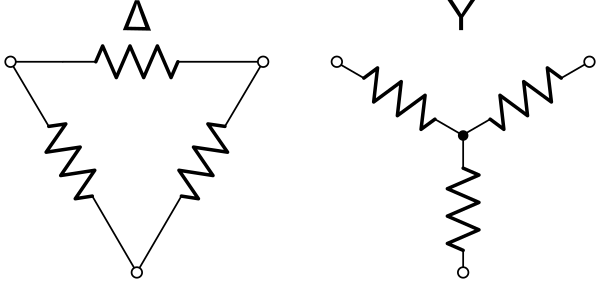
\includegraphics[height=1in]{figures/motor_winding.png}
		
		\caption[Motor Connection Configuration]{Motor Connection Configuration}
		
		\label{motor_configuration}
	\end{center}
\end{figure}

BLDC motors are typically connected in two wiring configurations: WYE (Y) or delta (\(\Delta \)), which can be seen in figure \ref{motor_configuration}. The RCTIMER GBM2804 utilizes the WYE (Y) configuration and will be analyzed as such. Due to the wiring of WYE systems, the neutral connection is typically unavailable for measurement on most motors. As a result, it is common to measure resistance by a line-line reading; however, in terms of motor control, it is the phase resistance and not the line-line resistance that is of importance. Converting between the phase and line-line resistance is quite simple and can be done by dividing the line-line resistance by two (equation \ref{eq:3.1}).

\begin{equation} \label{eq:3.1}
R = \frac{R_{LL}}{2}
\end{equation}

\subsection{Resistance Estimation}

In order to gather a good estimate for the phase resistance of the RCTIMER GBM2804 motor, the resistance was measured line-line across all three phases. Each set of motor leads were hooked up to a digital multimeter, and the values were tabulated for each phase component in table \ref{measured_motor_resistance}. An average was then calculated between the different line-line resistances to get the overall resistance of the motor.

\begin{table}[H]
	\begin{center}
		\caption{Measured motor resistance}
		\begin{tabular}[c]{ c c c }
			
			\textbf{A-B} & \textbf{A-C} & \textbf{B-C}\\
			
			\Xhline{2\arrayrulewidth}

			9.870 \(\Omega\)  & 9.900  \(\Omega\) & 9.950 \(\Omega\) \\
			
			\hline
			& \textbf{Average:} & 9.91 \(\Omega\) \\
			
			\Xhline{2\arrayrulewidth}
			\end{tabular}
			
			\label{measured_motor_resistance}
	\end{center}
\end{table}

Using equation \ref{eq:3.1}, it is then possible to find the overall phase resistance of the motor.

\begin{tcolorbox}[standard jigsaw,
	opacityback=0]
	\[R = 4.955 \approx 5 \Omega \]
	
\end{tcolorbox}

\section{Motor Torque Constant and Back EMF}
The motor torque constant (\(k_t\)) is a common parameter used in BLDC motors. It relates the armature current to the torque produced by a motor: \(T = k_T i \). Many methods exist to determine the torque constant, including relating the motor velocity constant \(k_v\), which is inversely related to the torque constant by \(k_T = \frac{1}{k_v} \), or by measuring the line-line back-emf voltage per phase (\(K_{e,p}\)). \(K_{e,p}\) is the peak value of the back-emf per angular velocity measured from line-neutral. However, since line-neutral is typically unavailable on most BLDC motors, the back-emf constant is often represented as a line measurement, \(K_{e}\). The overall torque constant can then be related to the line measurement back-emf voltage for sinusoidal type outputs by equation \ref{eq:3.2} or for trapezoidal outputs by equation \ref{eq:3.3}. \citep{5}. 

\begin{equation} \label{eq:3.2}
k_T = \frac{\sqrt{3}}{2} K_{e}
\end{equation}

\begin{equation} \label{eq:3.3}
k_T = K_{e}
\end{equation}

Because \(K_{e}\) can be experimentally determined, it is possible to find the overall motor torque constant for a BLDC motor. One simply needs to measure the line-line sinusoidal or trapezoidal back-emf voltage at various speeds to get a good estimate of \(K_{e}\). With equation \ref{eq:3.2} or \ref{eq:3.3}, \(k_T\) can then be determined.

\subsection{Estimating the Back EMF Constant}
In order to calculate the back-emf of the RCTIMER GBM2804 BLDC motor, an experiment had to be set up to measure the voltage generated by the motor. Three pieces of equipment were needed: an oscilloscope, the Motorlab, and a torque transmission shaft. The torque transmission shaft was a 3D printed part\footnote{Appendix \ref{Appendix:Key2} figure \ref{torque_transmission_shaft_drawing}} that allowed the Motorlab to spin the RCTIMER GBM2804 at a constant speed to generate a back voltage. A line-line voltage (peak-peak) was then read from the leads of the RCTIMER GBM2804 by an oscilloscope\footnote{Appendix \ref{Appendix:Key1} figure \ref{back_emf_measurement}}. The data collected is tabulated in table \ref{table3}.

\begin{table}[H] %ht
\begin{center}
\caption{Measured back voltage }
\begin{tabular}[c]{ c c c c }

\textbf{Speed (RPM)} & \textbf{Speed \(\omega_m\) (rad/s)} & \textbf{Peak-Peak Voltage (V)} & \textbf{Peak Voltage (V)}\\

\Xhline{2\arrayrulewidth}

\rowcolor{gray!20}
300  & 31.41  & 4.64 & 2.32\\


500 & 52.36 & 7.60 & 3.8\\

\rowcolor{gray!20}
1000 & 104.72 & 15.1 & 7.55\\


1500 & 157.10 & 22.0 & 11.0\\

\rowcolor{gray!20}
2000 & 209.44 & 30.0 & 15.0\\

\Xhline{2\arrayrulewidth}
\end{tabular}

\label{table3}
\end{center}
\end{table}

There is a fairly linear relationship between the peak voltage and speed. Due to this fact, \(K_{e}\) can be approximated from the slope of \(\frac{V}{\omega_m}\). The normal equation from the least-squares method was employed to find the best fit for the data in table \ref{table3}. Two matrices were constructed from the data, namely \(\matrva{V}\) and \(\matrva{\omega_m}\).

\begin{equation} \label{eq:3.4}
K_{e} = (\matrva{\omega_m \omega_m^T})^{-1} \matrva{\omega_m V^T}
\end{equation} 

From equation \ref{eq:3.4}, the back-emf constant was found to be: 
\[K_{e} = 0.0713 \quad \frac{V \cdot s}{rad} \]

To verify that \(K_{e}\) was the best fit to that data, \(K_{e}\) was plotted against the collected data in figure \ref{back_emf_plot}.

\begin{figure}[H]
	\centering
		\caption[Measured Back EMF vs Speed]{Measured Back EMF vs Speed}
		\label{back_emf_plot}
		% This file was created by matlab2tikz.
%
%The latest updates can be retrieved from
%  http://www.mathworks.com/matlabcentral/fileexchange/22022-matlab2tikz-matlab2tikz
%where you can also make suggestions and rate matlab2tikz.
%
\definecolor{mycolor1}{rgb}{0.00000,0.44700,0.74100}%
%
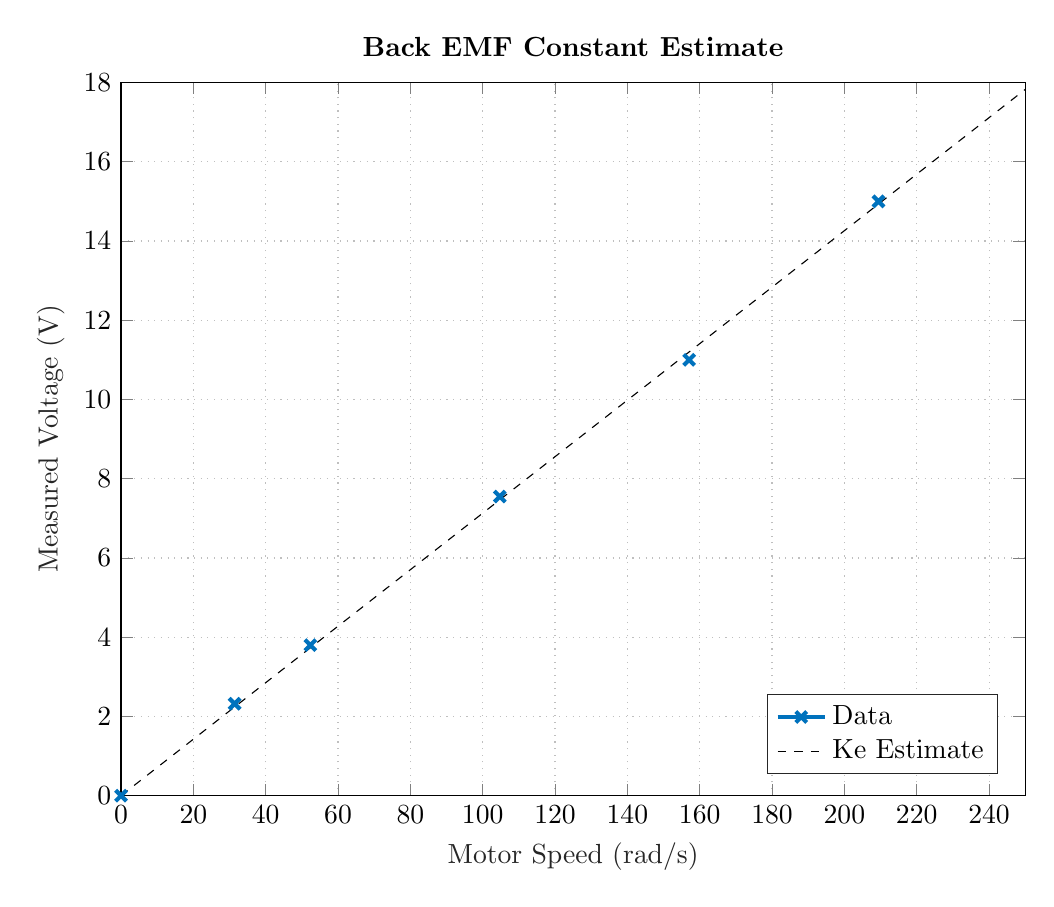
\begin{tikzpicture}

\begin{axis}[%
width=4.521in,
height=3.566in,
at={(0.758in,0.481in)},
scale only axis,
xmin=0,
xmax=250,
xlabel style={font=\color{white!15!black}},
xlabel={Motor Speed (rad/s)},
ymin=0,
ymax=18,
ylabel style={font=\color{white!15!black}},
ylabel={Measured Voltage (V)},
axis background/.style={fill=white},
title style={font=\bfseries},
title={Back EMF Constant Estimate},
xmajorgrids,
ymajorgrids,
grid style={dotted},
legend style={at={(0.97,0.03)}, anchor=south east, legend cell align=left, align=left, draw=white!15!black}
]
\addplot [color=mycolor1, line width=1.5pt, draw=none, mark size=2.8pt, mark=x, mark options={solid, mycolor1}]
  table[row sep=crcr]{%
0	0\\
31.4159265358979	2.32\\
52.3598775598299	3.8\\
104.71975511966	7.55\\
157.07963267949	11\\
209.43951023932	15\\
};
\addlegendentry{Data}

\addplot [color=black, dashed]
  table[row sep=crcr]{%
0	0\\
250	17.825\\
};
\addlegendentry{Ke Estimate}

\end{axis}
\end{tikzpicture}%
		
\end{figure}



Since the relationship between \(k_T\) and \(K_{e}\) is known by equation \ref{eq:3.2} and \ref{eq:3.3}, \(k_T\) can now be calculated.
\begin{tcolorbox}[
    standard jigsaw,
    opacityback=0]
\[k_T = 0.0617 \approx 0.06 \quad \frac{N \cdot m}{A} \quad [Sinusoidal]\]
\[k_T =  0.0713 \approx 0.07 \quad  \frac{N \cdot m}{A} \quad [Trapezoidal]\]
\end{tcolorbox}

\newpage
\section{Mass Moment of Inertia Estimation}
\label{mass_moment_of_inertia_estimation}
Mass moment of inertia (\(J\)) is the equivalent to mass in a rotational system (commonly referred to as angular mass). More formally, is it defined as \(J = \int r^2 dm\), where r is the distance to a mass from an axis of rotation.

The angular mass of the NERMLAB will be determined in two ways: approximating \(J\) through software modeling and approximating \(J\) through mathematical formulation. 

Multiple inertias will be referenced throughout this thesis, one being the base load inertia of the rotor, which is comprised of individual neodymium magnets held by an outer aluminum casing, and the second inertia being a simple steel washer. Most of section \ref{mass_moment_of_inertia_estimation} will be devoted to developing the base load inertia as it has a more complicated geometry than the simple washer. Because of this, the washer will be only developed in the section \ref{mathmematical_approximation_J}. Table \ref{measured_rotor_parameters} tabulates the various parameters that are referenced in all mass moment of inertia calculations.

\begin{table}[H] %ht
	\begin{center}
		\caption[Measured Inertia Parameters]{Measured Inertia Parameters}
		\begin{tabular}[c]{ l r }
			
			\textbf{Parameter} & \textbf{Value}\\
			
			\Xhline{2\arrayrulewidth}
			\rowcolor{gray!20}
			Magnet Thickness &  0.002 m\\
			
			Rotor Outer Radius &  0.0164 m\\
			
			\rowcolor{gray!20}
			Rotor Mass & 0.018 kg\\
			
			Washer Mass & 0.045 kg\\
			
			\rowcolor{gray!20}
			Washer Inner Radius & 0.0105 m\\
			
			Washer Outer Radius & 0.0253 m\\
			
			\Xhline{2\arrayrulewidth}
		\end{tabular}
		
		\label{measured_rotor_parameters}
	\end{center}
\end{table}

\subsection{Software Modeling of Mass Moment of Inertia}
\label{subsection_software_modeling}
\ac{CAD} software was utilized to construct a 3-D model of the neodymium magnets and aluminum casing. CAD software like SolidWorks has the ability to determine complex mass moment of inertias via numerical methods. Knowing the average density of neodymium ($7.3 - 7.5 \ \frac{g}{cm^3}$) and aluminum ($2.7 \ \frac{g}{cm^3}$), it is possible to numerically find an inertia ($J_s$) of the rotor.

\[J_s = 4.0842 \times 10^{-6} \ kg \cdot m^2\]


\subsection{Mathematical Approximation of Mass Moment of Inertia}
\label{mathmematical_approximation_J}
To simplify the mathematical analysis of the mass moment of inertia calculation of the angular mass of the NERMLAB, an engineering assumption will be made that the angular mass is a rotating ring mass. This assumption is valid for the particular motor used in this thesis, due to the fact that most of the mass is concentrated around the outside parameter of the motor. The outside ring mass of the motor contributes the most to the inertial load, so the mathematical formulation would result in the following equation:
\begin{equation}
\label{eq_J}
J_z = mr^2
\end{equation}

Knowing the outer radius of the rotor, it is possible to find the mathematical approximation of the rotor's inertia using equation \ref{eq_J}.

\[J_m = 4.8413 \times 10^{-6} \ kg \cdot m^2\]



\subsubsection{Washer Inertia}
Approximating the washer inertia is relatively straight forward as the geometry is simple to measure. As stated in subsection \ref{mathmematical_approximation_J}, the only dimensions that need measuring are the inner and outer radii, which are provided in table \ref{measured_rotor_parameters}.

With the measured radii results and mass properties from table \ref{measured_rotor_parameters}, the washer inertia can be easily approximated using equation \ref{eq_J}.

\[J_w = 2.8804 \times 10^{-5} \approx 3.0 \times 10^{-5}\ kg \cdot m^2 \]


\subsection{Lumped Mass Moment of Inertia}

\begin{equation}
\label{average_J_calculation}
J_r =  \frac{J_m + J_s}{2}
\end{equation}

Having two approximations for the inertia of the rotor, it is now possible to calculate an average between the two. Using the results from subsections \ref{mathmematical_approximation_J} and \ref{subsection_software_modeling}, and equation \ref{average_J_calculation}, the overall rotor inertia is found to be:

\[J_r =  4.4627 \times 10^{-6} \approx 4.5 \times 10^{-6} \ kg \cdot m^2 \]

For most of the experiments ran in this thesis, additional inertia is used to slow down the response of the system to allow a better visualization of what is happening when looking directly at the motor as it runs. For the total lumped inertia of the system, three steel washers are being used. Since all inertias in the system are rotating about the same axis, the total lumped inertia of the system is described by equation \ref{equation_lumped_inertia}.

\begin{equation}
\label{equation_lumped_inertia}
J = 3J_w + J_r
\end{equation}

\begin{tcolorbox}[
	standard jigsaw,
	opacityback=0]
	\[J = 9.45 \times 10^{-5} \ kg \cdot m^2 \]
\end{tcolorbox}


\section{Motor Inductance}
\label{section_motor_inductance}

The motor inductance is measured by building a simple circuit, which consists of a resistor in series with one of the motor's phase circuitry, as depicted in figure \ref{inductance_measurement}.

\begin{figure}[H]
	\caption[Inductance Measurement Circuit]{Inductance Measurement Circuit}
	\label{inductance_measurement}
	\centering
	% NERMLAB Inductance Measurement Circuit
	
\begin{circuitikz}
	\draw
	(0,0) to [sV, v=$V$, *-*] (0,6) 
	to [short] (2,6)
	to [L,l_=$L_m$,*-*] (2,4)
	to [R,l_=$R_m$,*-*] (2,2)
	to [R,l_=$R$,*-*]   (2,0)
	to [short] (0,0)
	(2,0) node[ground]{};
	
	\draw
	(2,6) to [short,l=$V_{source}$,-o] (4,6)
	(2,2) to [short,l=$V_{motor}$,-o] (4,2)
	(2,0) to [short,-o] (4,0)
	(4,6) to [open, v^>=$Ch. \ 1$,o-o] (4,2)
	(4,2) to [open, v^>=$Ch. \ 2$,o-o] (4,0);
\end{circuitikz}
	
	
	
	
%	\begin{circuitikz} 
%		\draw
%		(0,0) to [sV, v=$V$, *-*] (0,2) 
%		to [R, l=$12 k\Omega$] (2,2)
%		to [R, l=$R$] (4,2)
%		to [L, l=$L$] (6,2)
%		to (6,0) to  (6,2) -- (6,0) -- (0,0);
		
%		\draw
%		(0,2) to [short=$Oscilliscope$,-o] (0,3);
		
%		\draw
%		(2,2) to [short,*-o] (2,3);
		
%		\node[draw,text width=2.15cm] at (1,3.45){Oscilloscope};
%		\node[draw,text width=3cm] at (4,1.4){Motor Circuitry};

%	\end{circuitikz}

\end{figure}

A function generator is required for this experiment to generate a variable frequency sin wave across the external resistor and motor. Knowing that figure \ref{inductance_measurement} is a simple voltage divider, it is possible to arrive at equation \ref{inductance_equation} using the relationship $\lvert V_{motor} \rvert = \frac{1}{2} \lvert V_{source} \rvert$, where $f$ is the driving frequency of the sinusoid. Then, the voltages of two outputs are monitored on seperate channels on an oscilloscope, and the sinusoidal frequency is increased until the motor output's voltage reaches one half of that of the source voltage.


\begin{equation}
\label{inductance_equation}
L = \frac{R\sqrt{3}}{2\pi f}
\end{equation}

\subsection{Inductance Estimate}
With the outlined procedure developed in the previous section (\ref{section_motor_inductance}), three resistors were measured, and the voltages across each junction were tabulated when an appropriate frequency was reached. Table \ref{inductance_experiment_table} hosts the experimental results, along with the calculated average inductance that was found from equation \ref{inductance_equation}.

\begin{table}[H] %ht
	\begin{center}
		\caption[Inductance Experiment]{Inductance Experiment}
		\begin{tabular}[c]{l c c c r}
			
			 \textbf{Resistance ($\Omega$)} & \textbf{$V_{source}$ ($V$)} & \textbf{$V_{motor}$ ($V$)} & \textbf{Frequency ($kHz$)} & \textbf{Inductance ($H$)}\\
			\Xhline{2\arrayrulewidth}


			\rowcolor{gray!20}
		    22   & 0.392 & 0.176 & 8.34  & $7.27 \times 10^{-4}$\\
			

		    98.4 & 1.04 & 0.507  & 34.4  & $7.88 \times 10^{-4}$\\
			
			\rowcolor{gray!20}
			461  & 1.88 & 0.920  & 167.5 & $7.58 \times 10^{-4}$\\
			
			\hline
		     & &  & \textbf{Average:} & \textbf{$7.58 \times 10^{-4}$}\\
			
			\Xhline{2\arrayrulewidth}
		\end{tabular}
		
		\label{inductance_experiment_table}
	\end{center}
\end{table}

\begin{tcolorbox}[
	standard jigsaw,
	opacityback=0]
	\[L = 7.58 \times 10^{-4} \ H \]
\end{tcolorbox}

\section{Viscous Friction}
\label{viscous_friction}

Section \ref{viscous_friction} will not detail the process conducted to determine the viscous friction of the NERMLAB, as this will be discussed in chapter \ref{chp4}, where a laboratory has already been developed for students to estimate this coefficient. For the sake of completeness the result will be provided below.

\begin{tcolorbox}[
	standard jigsaw,
	opacityback=0]
	\[b = 5.3 \times 10^{-4} \ N\cdot m\cdot s\]
\end{tcolorbox}

